\chead{CHAPITRE 3. SPRINT 1 : Authentification & Gestion des Identités}

\chapter{Sprint 1: Authentification et Gestion des Identités}
\renewcommand{\mtctitle}{Sommaire}
\minitoc
	\newpage

\section*{Introduction}
\addcontentsline{toc}{section}{\protect\numberline{}Introduction}
Le coup d'envoi technique de \textbf{SmartRec} se concrétise à travers ce premier sprint, dont la vocation première est de sécuriser l'accès à la plateforme et de structurer l'écosystème utilisateur. Dans les pages qui suivent, nous explorerons comment l'architecture Salesforce a été exploitée pour bâtir un système d'authentification robuste. Nous détaillerons le passage du backlog fonctionnel à la mise en œuvre concrète des portails recruteurs et candidats, en illustrant chaque avancée par des visuels issus de l'environnement de production.

\section{Objectifs du Sprint}
L’enjeu majeur de cette itération initiale réside dans la segmentation fine des accès. Il s'agit non seulement de permettre une connexion sécurisée, mais surtout de garantir que chaque acteur — qu'il s'agisse d'un administrateur PwC ou d'un candidat externe — interagisse avec une interface adaptée à ses prérogatives métier, grâce à la flexibilité d'Experience Cloud.


\section{Spécification des besoins}
\par Dans cette section, nous présentons le diagramme des cas d’utilisation du sprint ainsi que le backlog associé. L'objectif est de définir clairement les interactions entre les utilisateurs (Administrateur, Recruteur et Candidat) et la plateforme Salesforce.
\subsection{Diagramme cas d’utilisation du Sprint 1}

 \begin{figure}[H]
    \centering
    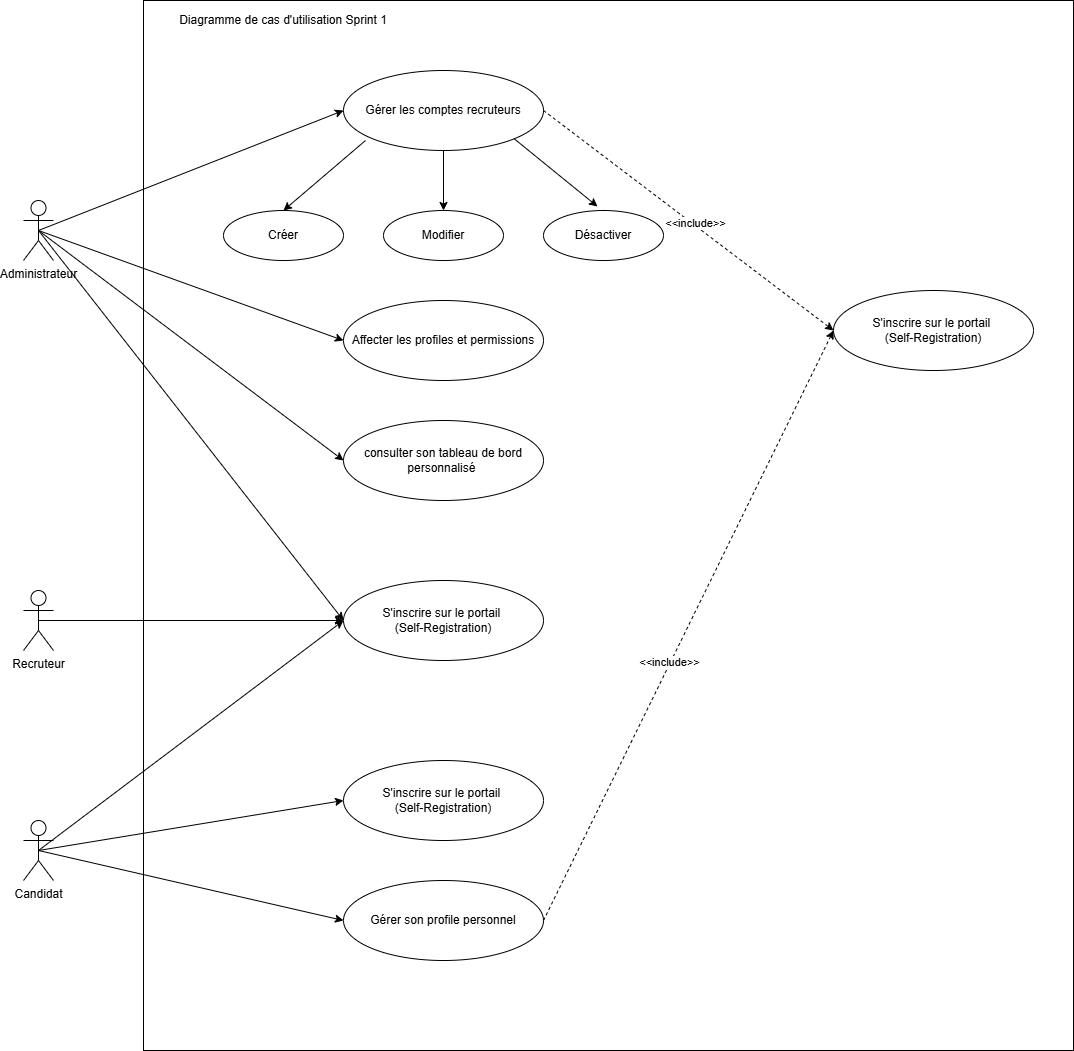
\includegraphics[width=12cm, height=12cm]{Figures/use case 1.png}
    \caption{Diagramme de cas d’utilisation du sprint 1}
    \label{fig:Diagramme de cas d’utilisation du sprint 0}
\end{figure}


\subsection{ Sprint Backlog du sprint 1}
Le tableau ci-dessous présente le sprint backlog établi pour le premier sprint. Il récapitule les différentes user stories sélectionnées, accompagnées de leurs identifiants uniques, ainsi que les tâches techniques à réaliser pour chacune. Ce tableau permet d’avoir une vision claire et structurée du travail prévu, en facilitant la planification, la répartition des responsabilités et le suivi de l’avancement tout au long du sprint.
\begin{table}[H]
\caption{Backlog du sprint 1 : Gestion des utilisateurs et accès}
    \centering
    \begin{tabular}{|p{1cm}|p{8cm}|p{8cm}|}
    \hline
    \textbf{ID} & \textbf{User Story} & \textbf{Tâches techniques (Salesforce)} \\
    \hline
    US-1 & En tant qu'administrateur, je veux créer les comptes des recruteurs afin de leur donner accès au CRM.
    & 
    \begin{itemize}[leftmargin=*]
    \item Configuration des profils et rôles Salesforce.
    \item Création de l'objet utilisateur interne.
    \item Attribution des Permission Sets.
    \end{itemize} \\
    \hline
    US-2 & En tant qu'administrateur, je veux gérer (modifier/désactiver) les comptes utilisateurs. & 
    \begin{itemize}[leftmargin=*]
    \item Configuration des Layouts de page utilisateur.
    \item Mise en place de flux d'automatisation (Flows).
    \end{itemize} \\
    \hline
    US-3 & En tant qu'administrateur, je veux consulter la liste complète des utilisateurs internes pour superviser les accès.  & 
    \begin{itemize}[leftmargin=*]
    \item Configuration des vues de liste personnalisées.
    \item Mise en place de filtres par profil (Recruteur Platform).
    \end{itemize} \\
    \hline
    US-4 & En tant qu'utilisateur, je veux accéder à un tableau de bord Salesforce pour visualiser mes indicateurs clés.& 
    \begin{itemize}[leftmargin=*]
    \item Création de rapports et tableaux de bord natifs.
    \item Personnalisation de la page d'accueil Lightning.
    \end{itemize} \\
    \hline
    US-6 & En tant que candidat, je veux créer un compte sur le portail pour postuler aux offres.& 
    \begin{itemize}[leftmargin=*]
    \item Activation du portail Experience Cloud.
    \item Configuration du "Self-Registration" (inscription libre).
    \item Mapping automatique Candidat/Contact.
    \end{itemize} \\
    \hline
    US-7 & En tant que candidat, je veux mettre à jour mon profil et mes informations personnelles.& 
    \begin{itemize}[leftmargin=*]
    \item Développement d'un formulaire LWC pour l'objet Contact/Candidat.
    \item Gestion de la persistance des données via Apex DML.
    \end{itemize} \\
    \hline
    \end{tabular}
    \label{tab:user_stories_sprint1}
\end{table}

\section{Analyse des besoins}
Avant de traduire les exigences fonctionnelles en modèles techniques, il est primordial de décortiquer les parcours utilisateurs identifiés dans le backlog. Cette étape d'analyse textuelle permet de clarifier les règles de gestion et les comportements attendus du système Salesforce face aux sollicitations des acteurs.

\subsection{Description détaillée des cas d'utilisation}
        \begin{itemize}
        \item \textbf{Cas d'utilisation "Gérer les comptes recruteurs" :} La table 3.2 formalise le processus d'administration des utilisateurs internes au sein de l'organisation.
    \end{itemize}
    \begin{table}[H]
    \caption{Description textuelle du cas d'utilisation "Gérer les comptes recruteurs"}
    \centering
    \begin{tabular}{|c|p{12cm}|}
    \hline
    \textbf{Titre} & Gérer les comptes recruteurs \\
    \hline
    \textbf{Objectif} & Octroyer, modifier ou révoquer l'accès aux modules de recrutement pour les collaborateurs PwC. \\
    \hline
    \textbf{Acteur}& Administrateur\\
    \hline
    \textbf{Pré-condition} & Session administrateur active avec privilèges de gestion des utilisateurs. \\
    \hline
    \textbf{Post-condition} & Les privilèges d'accès sont immédiatement mis à jour dans l'annuaire Salesforce. \\
    \hline
    \textbf{Scénario nominal} & 1. L'administrateur se rend dans l'espace de gestion des utilisateurs. \newline
    2. Il définit le type d'utilisateur et saisit ses informations d'identité. \newline
    3. Il valide les paramètres de sécurité. \newline
    4. Le système déclenche l'envoi d'un e-mail d'activation au nouvel utilisateur. \\
    \hline
    \end{tabular}
    \label{tab:uc_accounts}
\end{table}




\begin{itemize}
        \item \textbf{Cas d'utilisation "Gérer les permissions et profils" :} La table 3.3 présente la description textuelle du cas d'utilisation relatif à la gestion des droits d'accès.
    \end{itemize}
    \begin{table}[H]
    \caption{Description textuelle du cas d’utilisation "Gérer les permissions"}
    \centering
    \begin{tabular}{|c|p{12cm}|}
    \hline
    \textbf{Titre} & Gérer les permissions et profils \\
    \hline
    \textbf{Objectif} & Permettre à l’administrateur d’attribuer des profils et Permission Sets spécifiques aux recruteurs. \\
    \hline
    \textbf{Acteur}& Administrateur\\
    \hline
    \textbf{Pré-condition} & L'utilisateur doit exister dans l'organisation Salesforce. \\
    \hline
    \textbf{Post-condition} & L'utilisateur dispose des accès restreints selon son rôle métier.\\
    \hline
    \textbf{Scénario nominal} & 1. L’administrateur accède à la configuration (Setup) de Salesforce. \newline
    2. Il recherche l'utilisateur cible. \newline
    3. Il sélectionne le profil adéquat (ex: Recruteur Standard). \newline
    4. Il affecte les ensembles de permissions (Permission Sets) nécessaires. \\
    \hline
    \end{tabular}
    \label{tab:uc_permissions}
\end{table}
\begin{itemize}
        \item \textbf{Cas d'utilisation "Consulter le tableau de bord" :} La table 3.4 décrit l'accès aux indicateurs de recrutement.
    \end{itemize}
    \begin{table}[H]
    \caption{Description textuelle du cas d’utilisation "Consulter le tableau de bord"}
    \centering
    \begin{tabular}{|c|p{12cm}|}
    \hline
    \textbf{Titre} & Consulter le tableau de bord de recrutement \\
    \hline
    \textbf{Objectif} & Permettre au recruteur de visualiser les statistiques clés (offres actives, candidatures reçues). \\
    \hline
    \textbf{Acteur}& Recruteur \\
    \hline
    \textbf{Pré-condition} & Le recruteur doit être authentifié sur l'application Salesforce. \\
    \hline
    \textbf{Post-condition} & Les rapports et graphiques de performance sont affichés en temps réel.\\
    \hline
    \textbf{Scénario nominal} & 1. Le recruteur accède à la page d'accueil de SmartRec. \newline
    2. Le système charge les composants LWC de statistiques. \newline
    3. Le recruteur visualise le nombre total de candidatures et leur répartition par statut. \\
    \hline
    \end{tabular}
    \label{tab:uc_dashboard}
\end{table}






\section{Conception}
\hspace{0.5cm}\textbf{Cette section détaille la phase de conception technique propre aux fonctionnalités du premier sprint. En nous appuyant sur le diagramme de classes global présenté au chapitre précédent (Chapitre 2, Figure 2.X), nous nous focalisons ici sur la modélisation dynamique. À travers des diagrammes de séquences, nous illustrons les interactions fluides entre les composants LWC, les contrôleurs Apex et les objets standards de Salesforce (User, Contact, Profile) mis en œuvre lors de l'inscription et de la gestion des identités.}








\subsection{Modélisation de la dynamique (Diagrammes de séquences)}
Pour illustrer la cinématique des échanges entre les différents composants du système, nous avons élaboré des diagrammes de séquences. Ces derniers mettent en lumière la collaboration entre les interfaces LWC, les contrôleurs Apex et la base de données. Le scénario ci-dessous se concentre sur l'un des flux les plus critiques du Sprint 1 : la création autonome d'un compte candidat.

\subsubsection{Diagramme de séquence : Création d'un compte candidat}
Cette vue détaille la chronologie des messages et des traitements lors de l'inscription d'un nouvel utilisateur sur le portail Experience Cloud.


\begin{figure}[H]
\centering
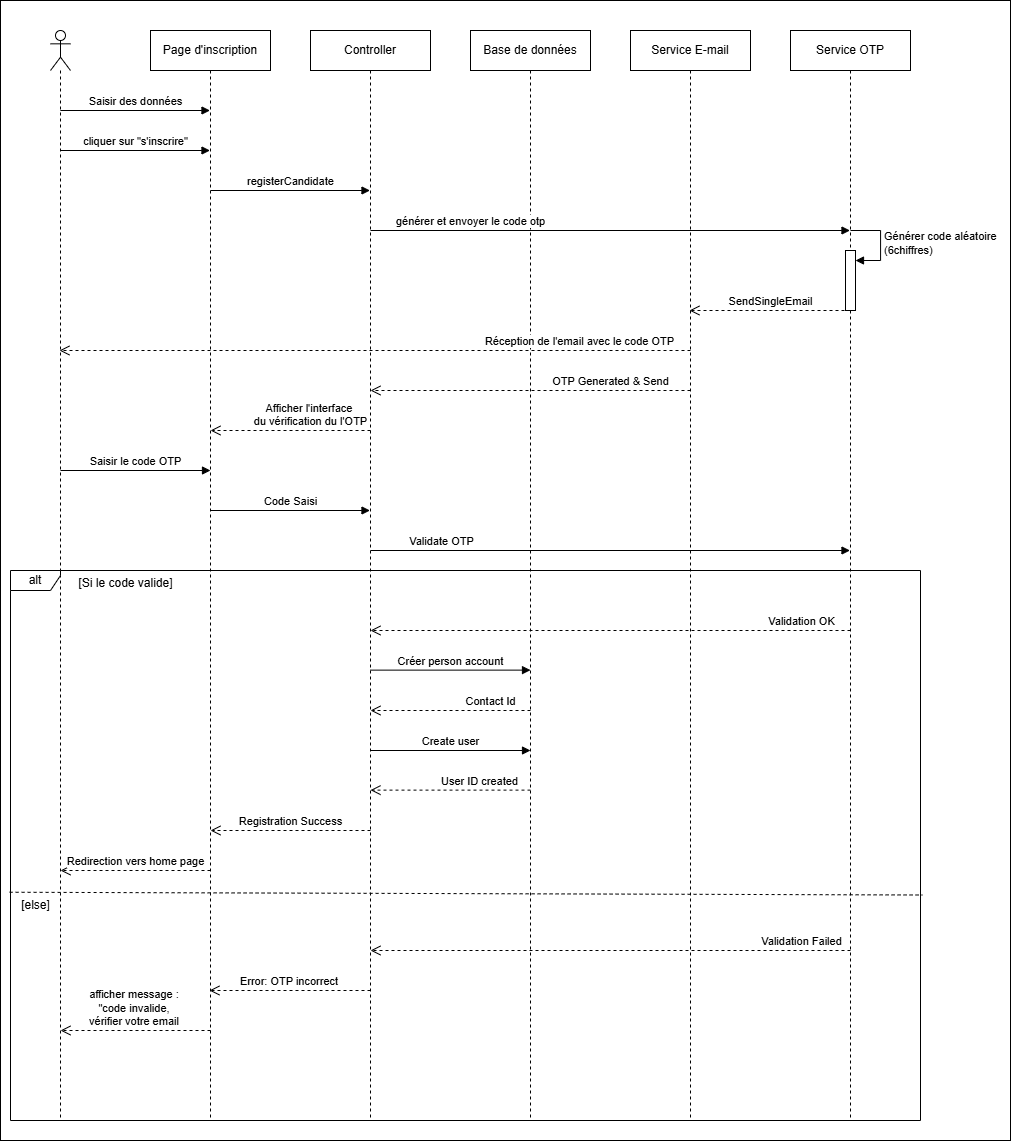
\includegraphics[width=18cm, height=19cm]{Figures/seq1.png}
\caption{Diagramme de séquence ”Créer un compte”}
\label{schema1}
\end{figure}
 




\section{Réalisation : interfaces utilisateur sur Salesforce}
Dans le cadre de ce sprint, les interfaces ont été réalisées en s'appuyant sur les standards de la plateforme Salesforce (Lightning Design System - SLDS). Cette section présente les vues principales de SmartRec, incluant les consoles d'administration et le portail Experience Cloud dédié aux candidats.


\vspace{5mm}
\begin{itemize}
    \begin{itemize}
         \item \textbf{Tableau de bord Recruteur (Lightning Experience) :} Le tableau de bord offre une vue d’ensemble en temps réel sur les indicateurs clés du recrutement : nombre d'offres actives, total de candidatures reçues et répartition des candidats par étape du processus. Il s'appuie sur les composants graphiques natifs de Salesforce.
         \begin{figure}[H]
             \centering
             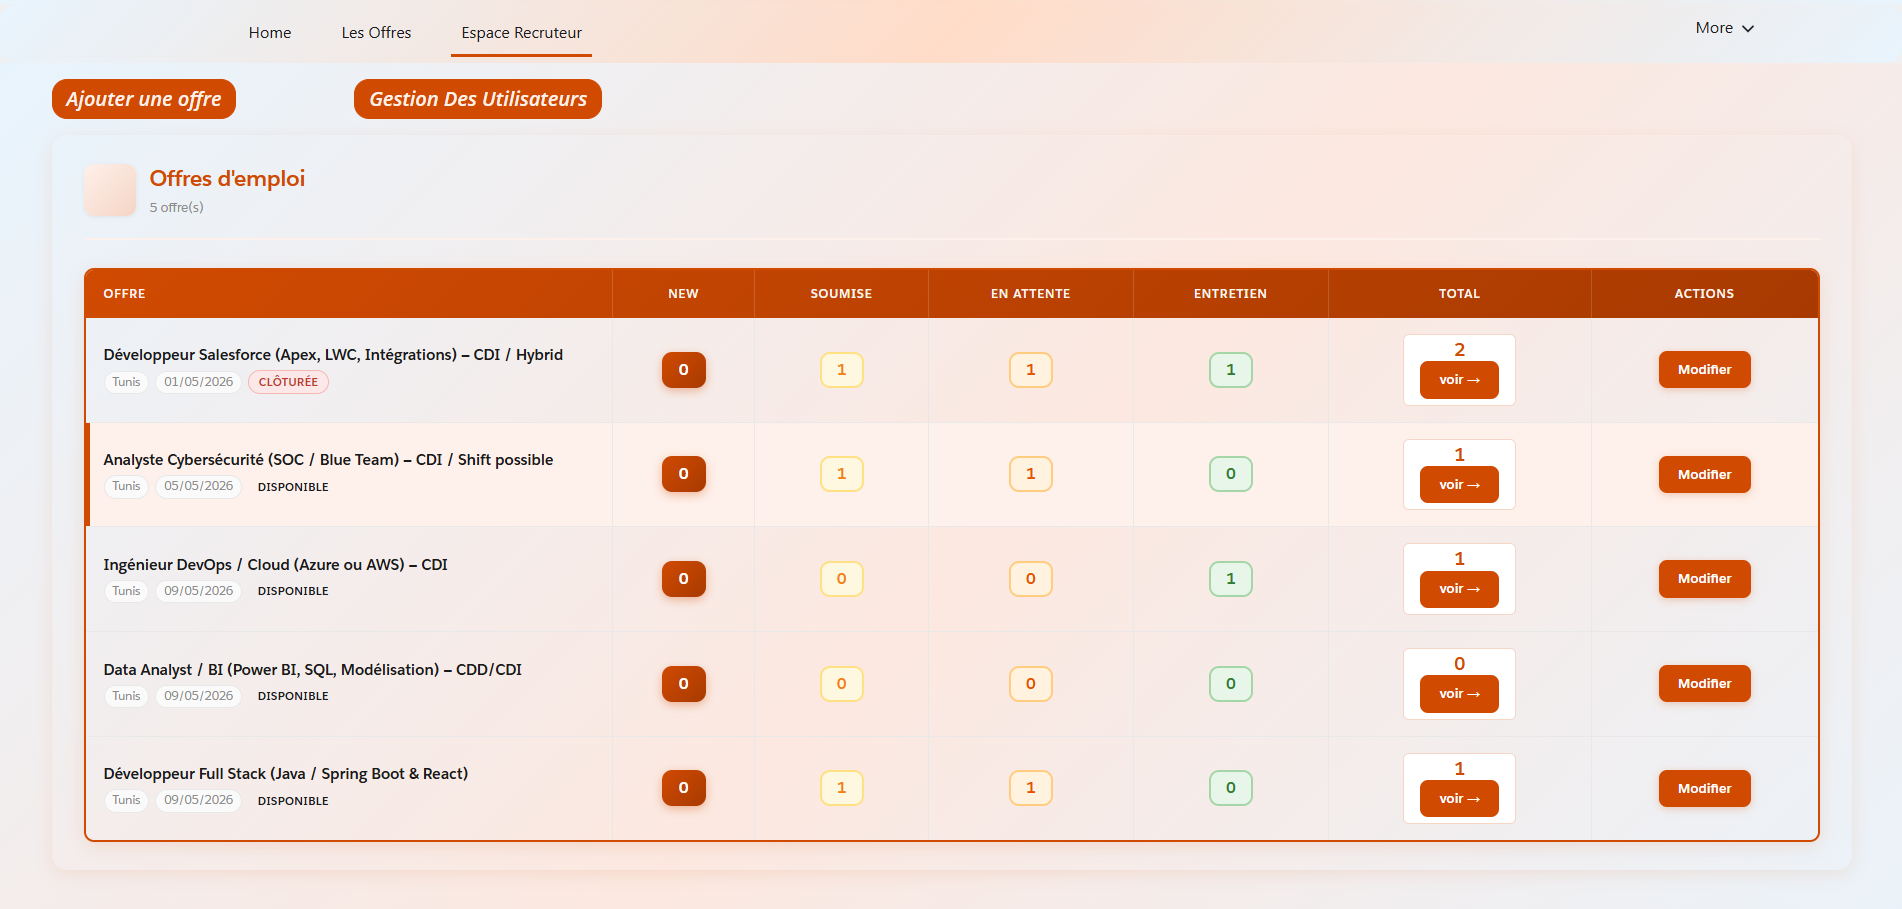
\includegraphics[width=\textwidth]{Figures/admindashbo.png}
             \caption{Tableau de bord de gestion (Lightning Experience)}
         \end{figure}
        \end{itemize}
    \begin{itemize}
        \item \textbf{Console d'Administration Salesforce (Setup) :} L'administrateur ne dispose pas d'une interface sur mesure ; il exploite la puissance du \textit{Setup} standard de Salesforce pour gérer les utilisateurs. C'est ici qu'il crée les comptes recruteurs en leur affectant le profil \textbf{Recruteur Platformdonc}.
         \begin{figure}[H]
             \centering
             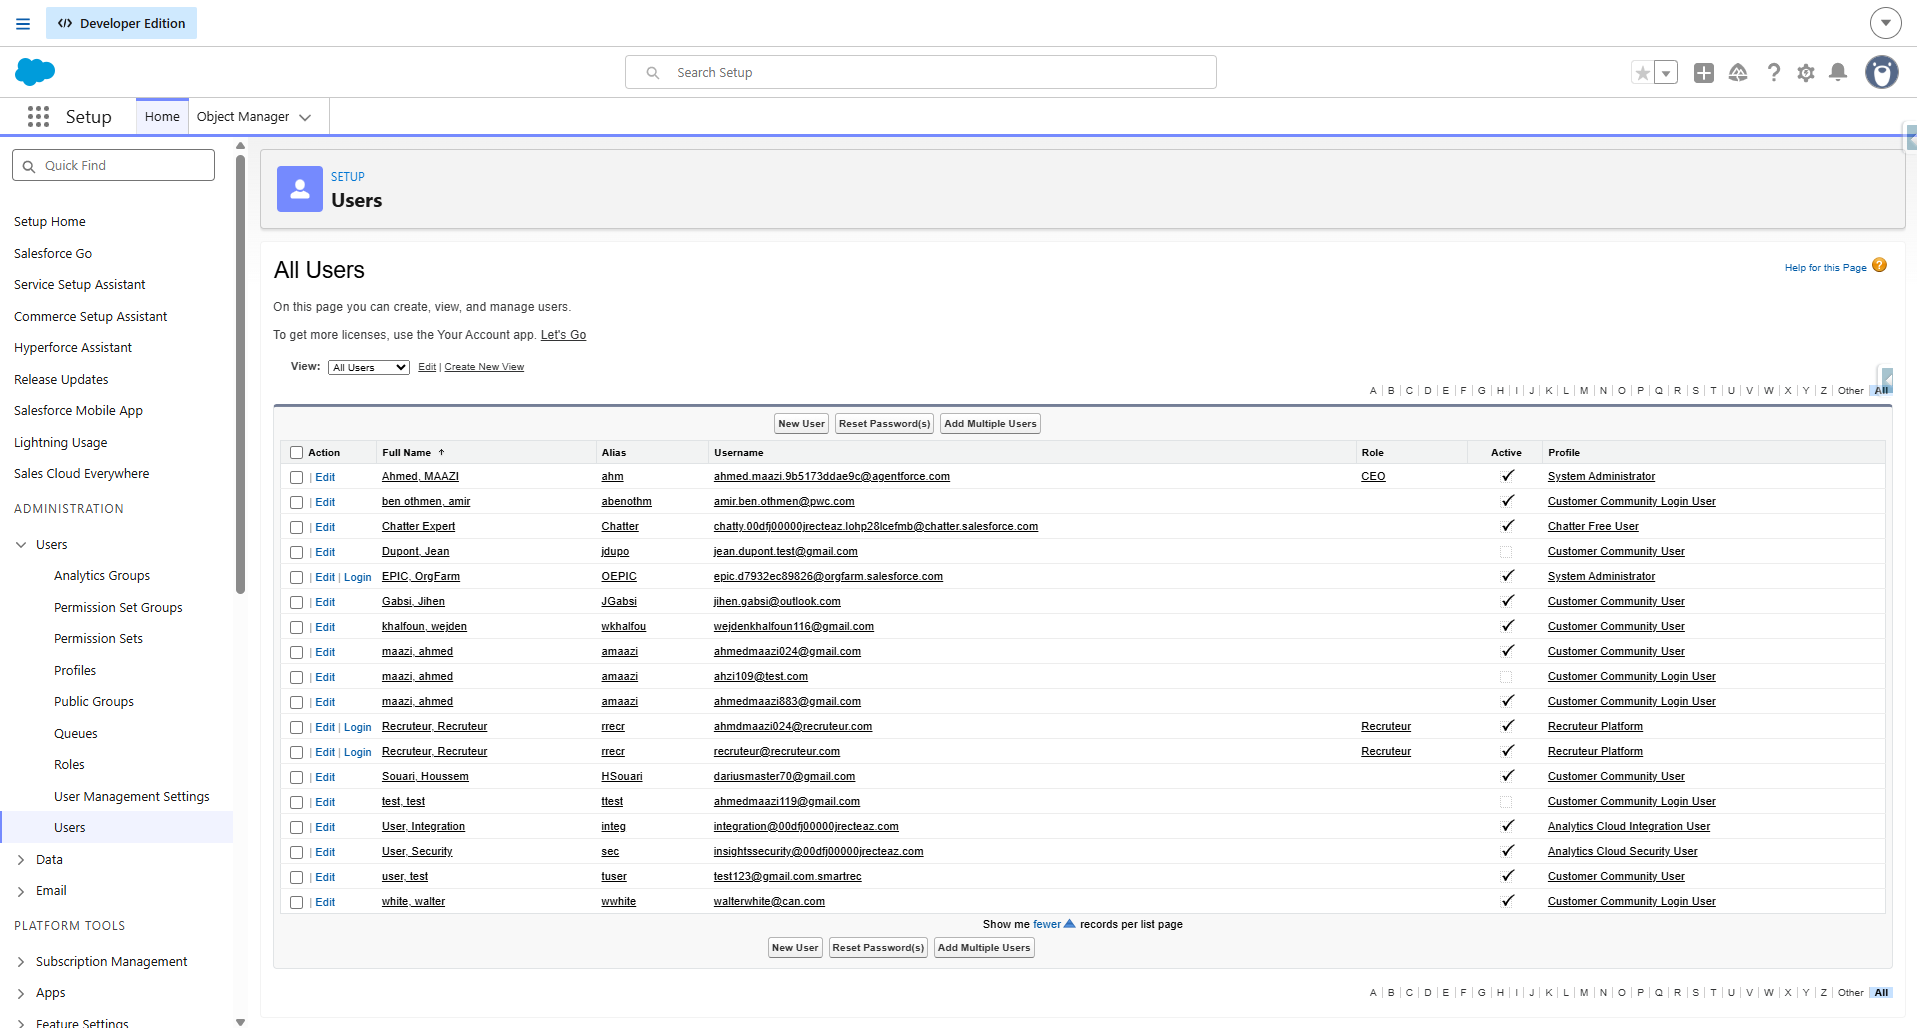
\includegraphics[width=\textwidth]{Figures/adminadduser1.png}
             \caption{Console de configuration standard pour la gestion des utilisateurs}
         \end{figure}
      \end{itemize}
\end{itemize}

\begin{itemize}
      \item\textbf{Suivi des candidatures par offre (Console Recruteur) :} 
Cette interface, au cœur de l'activité du recruteur, permet de consulter les détails d'une offre spécifique et de lister instantanément les candidats associés, facilitant ainsi le pilotage du workflow de recrutement.
          \begin{figure}[H]
              \centering
              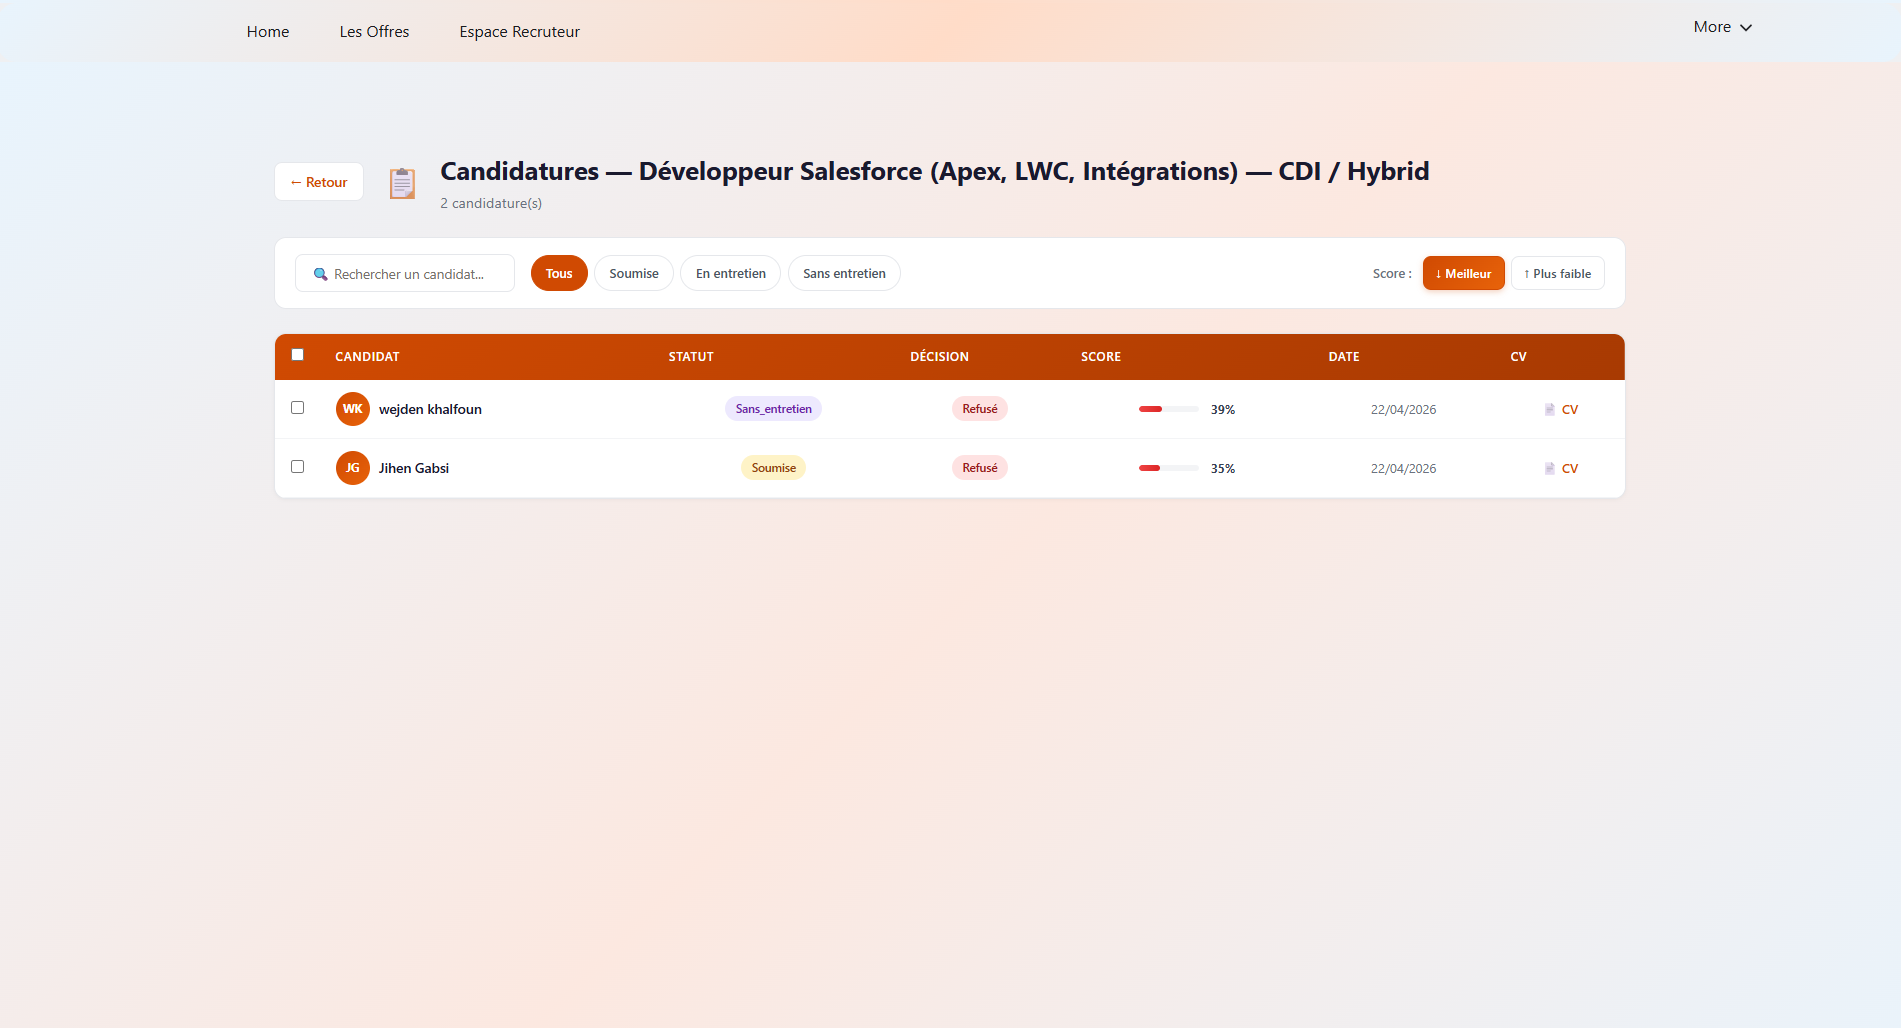
\includegraphics[width=\textwidth]{Figures/admintache.png}
              \caption{Interface de gestion des candidatures liées à une offre}
          \end{figure}
      \end{itemize}
\begin{itemize}
     \item\textbf{Interface d'inscription du candidat (Experience Cloud) :} 
Interface développée pour permettre aux nouveaux candidats de s'enregistrer de manière autonome. Elle valide les informations saisies et crée automatiquement un enregistrement de type Contact lié au compte utilisateur.
         \begin{figure}[H]
             \centering
             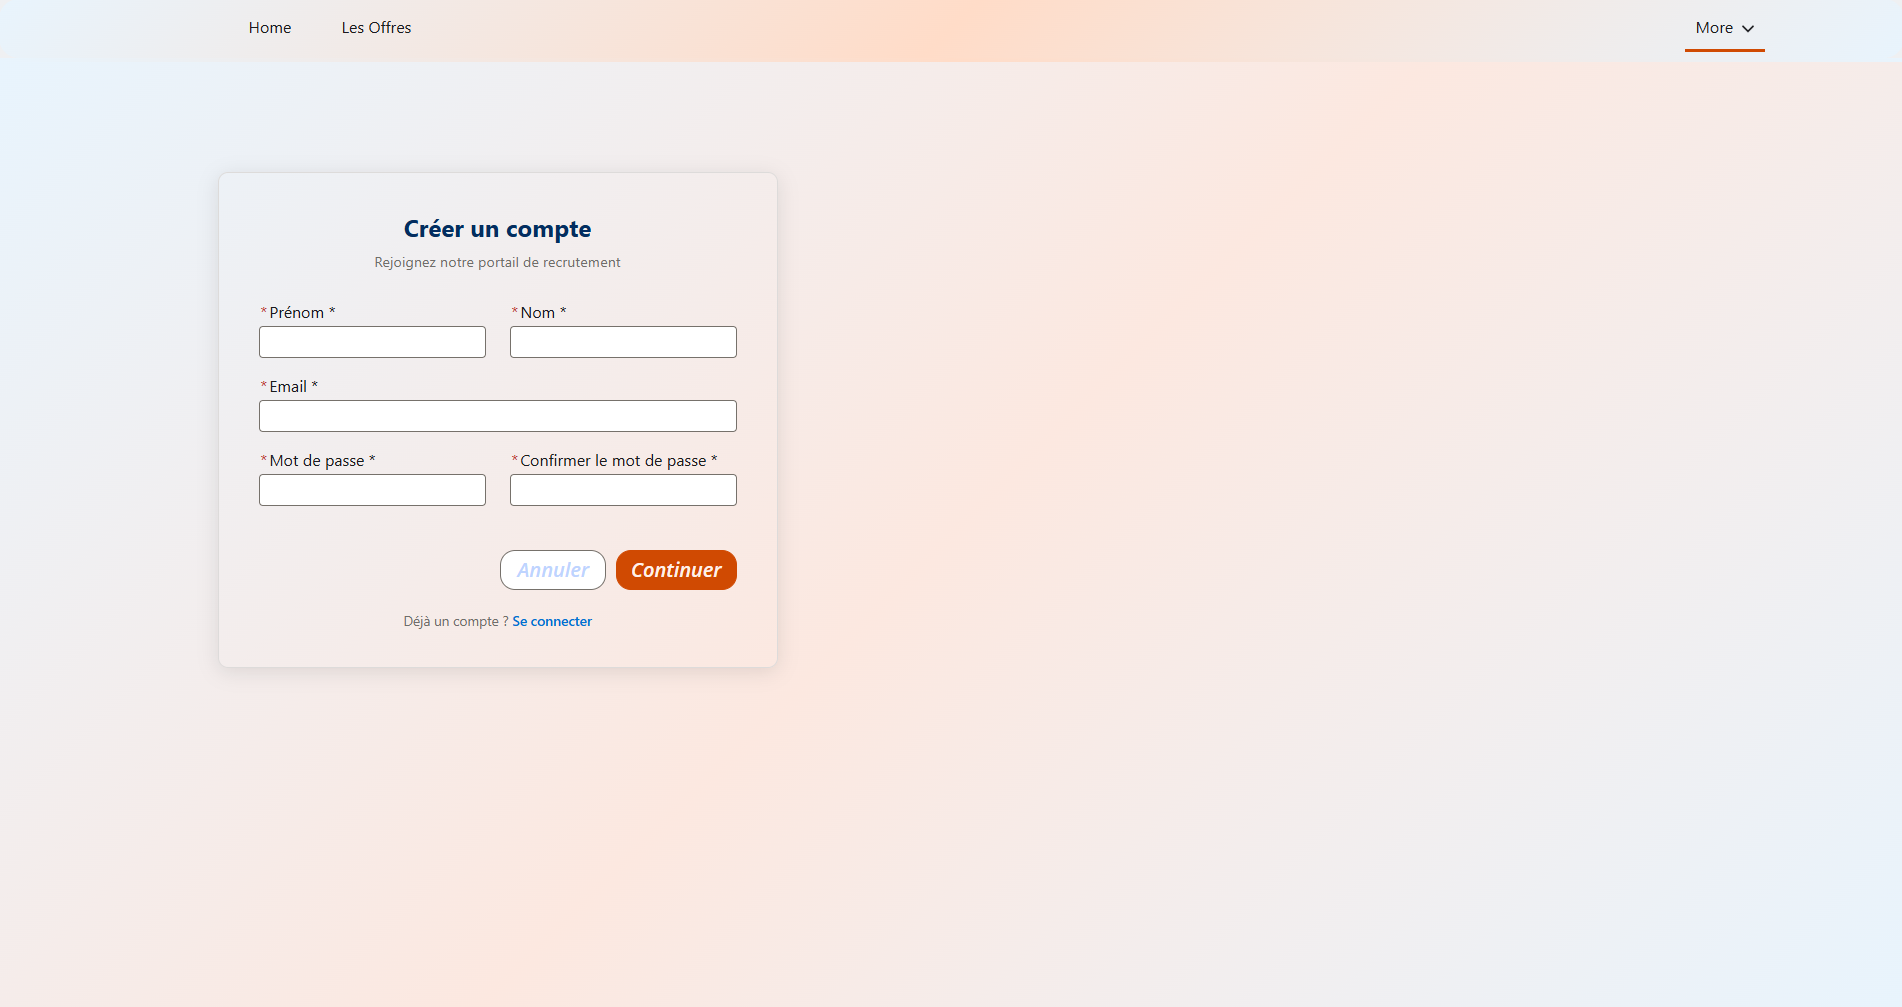
\includegraphics[width=\textwidth]{Figures/candidatinscri.png}
             \caption{Portail Candidat - Interface d'inscription}
         \end{figure}
     \end{itemize}
\begin{itemize}
      \begin{itemize}
          \item \textbf{Espace Candidat et Gestion du Profil :} Le portail offre une vue d'ensemble personnalisée où le candidat peut suivre l'état de ses candidatures et mettre à jour ses informations de profil (compétences, expériences) via des composants LWC dédiés.
          \begin{figure}[H]
              \centering
              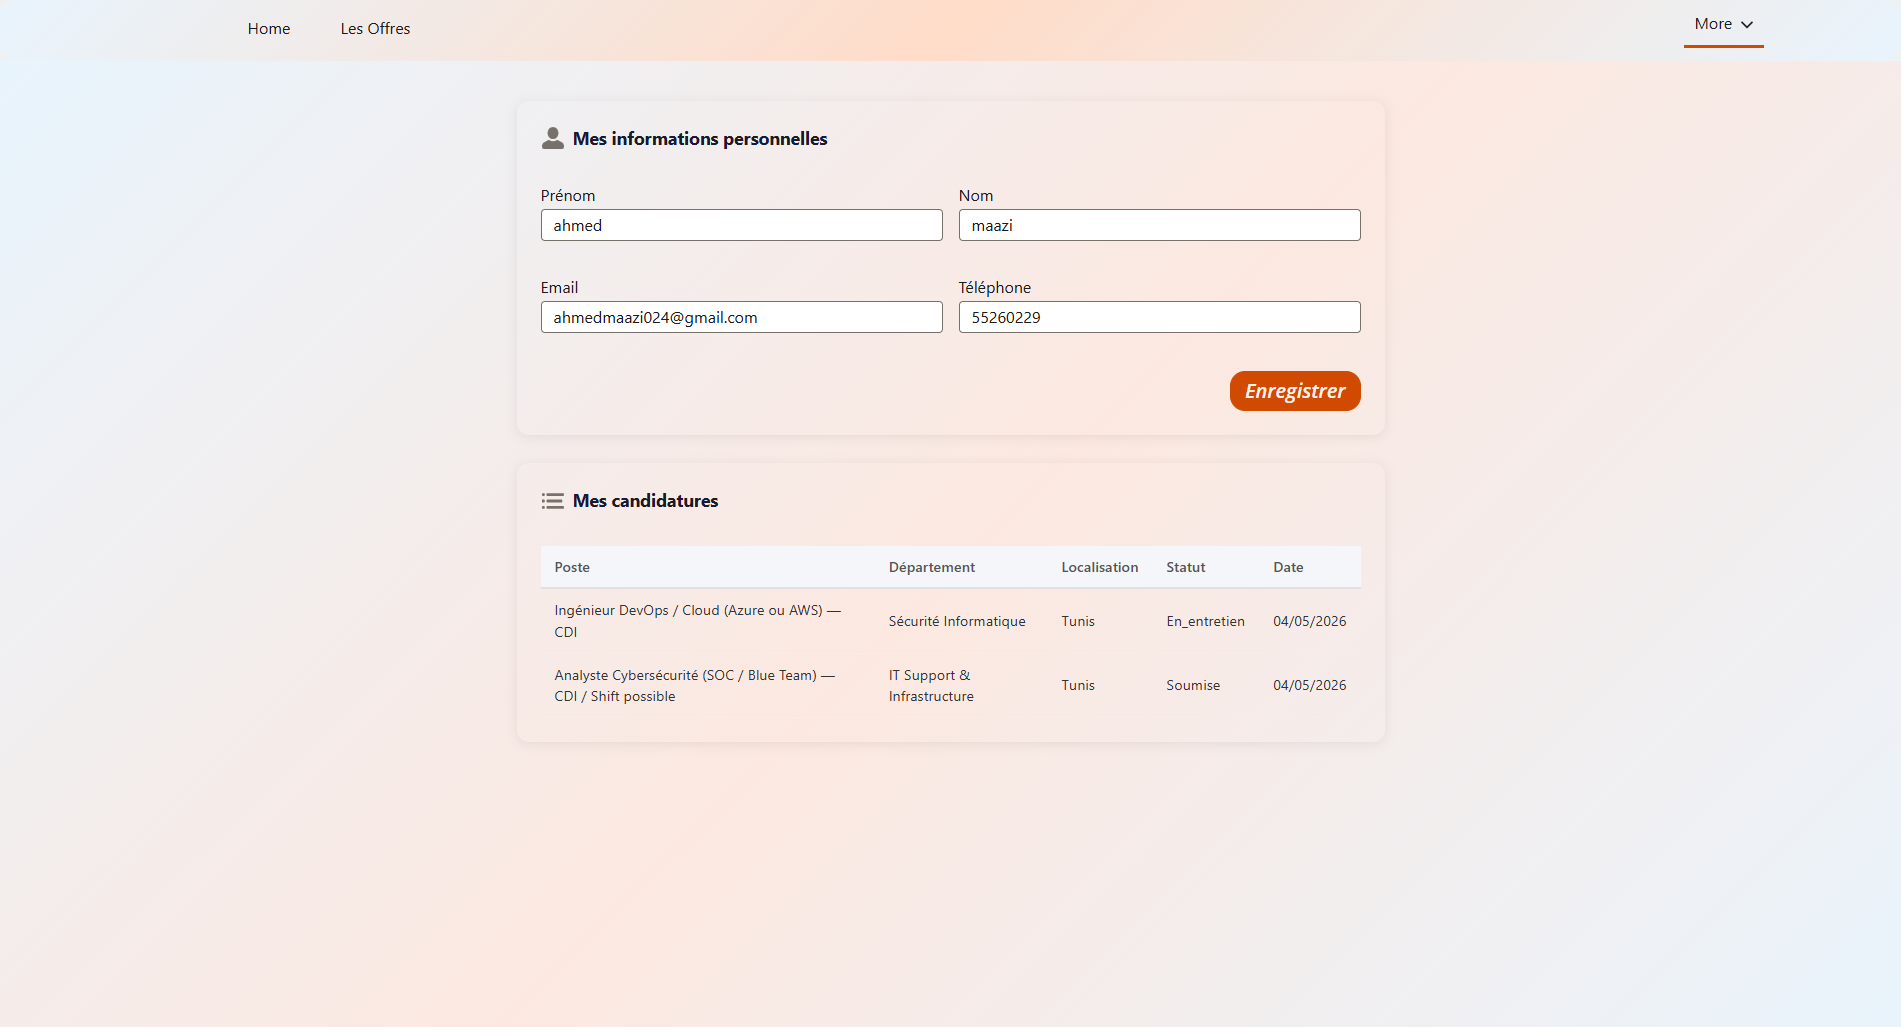
\includegraphics[width=\textwidth]{Figures/candidatprofil.png}
              \caption{Interface de gestion du profil candidat (LWC)}
          \end{figure}
      \end{itemize}
\end{itemize}



\section*{Conclusion}
\addcontentsline{toc}{section}{\protect\numberline{}Conclusion}
En définitive, ce premier sprint a permis de transformer une vision théorique de la sécurité en une infrastructure fonctionnelle sur Salesforce. En orchestrant les profils et les droits d'accès, nous avons créé un environnement de confiance, prêt à supporter les processus métiers complexes. Ce socle technique étant désormais stabilisé, le chapitre suivant se penchera sur le moteur même de SmartRec : la gestion automatisée du cycle de recrutement et l'analyse sémantique des profils.

 